As outlined in the main structure of this chapter, neural networks play a central role in modern machine learning.
Before diving into specific architectural types or training procedures, we begin this chapter with a high-level introduction to the basic concept of neural networks.
The goal is to provide an intuitive understanding of how they operate as function approximators by passing data through layers of interconnected units.
After this conceptual overview, we discuss common activation and loss functions, formalize the training process, and conclude the chapter with an overview of different neural network architectures.

Every artificial neuron receives one or more real-valued inputs and produces a single output.
This output is then passed on to other neurons in the network. 
At its core, an artificial neuron performs an affine transformation of the input followed by a non-linear activation function.

%To explain an artificial neuron, we follow Stevens et al. \cite{antiga_deep_2020}.
%A single artificial neuron takes an input vector $x=(x_1,x_2,\dots x_n)^\top \in \mathbb{R}^n$, applies a weighted sum with weights $w=(w_1,w_2,\dots,w_n)\in \mathbb{R}^n$, adds a bias term $b\in \mathbb{R}$ and passes the result through an activation function $\sigma$. 
%The output $y\in \mathbb{R}$ is given by:
%    \[y := \sigma(w^\top x+b).\]
%Figure \ref{fig:artNeuron} shows an artificial neuron.
To explain an artificial neuron, we follow Stevens et al.~\cite{antiga_deep_2020}.  
A single artificial neuron takes an input vector \( x = (x_1, x_2, \dots, x_n)^\top \in \mathbb{R}^n \), applies a weighted sum with weights \( w = (w_1, w_2, \dots, w_n) \in \mathbb{R}^n \), adds a bias term \( b \in \mathbb{R} \), and passes the result through an activation function \( \sigma \).  
The output \( y \in \mathbb{R} \) is given by:
\[
y := \sigma(w^\top x + b).
\]
This defines a function \( f \colon \mathbb{R}^n \to \mathbb{R} \), where the image \( \operatorname{Im}(f) \) depends on the choice of activation function \( \sigma \).  
Typical activation functions and their properties are discussed in detail in Section~\ref{ActFunc}.  
Figure~\ref{fig:artNeuron} shows an artificial neuron.




\begin{figure}[h]
    \centering
    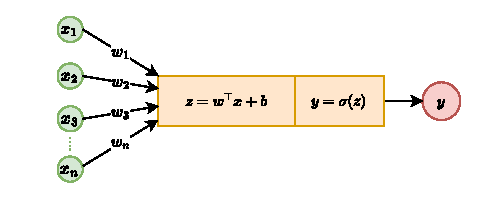
\includegraphics[width=0.7\linewidth]{Abschlussarbeit/Pictures/ArtificialNeuron_output.pdf}
    \caption{Illustration of a neural networks artificial neuron}
    \label{fig:artNeuron}
\end{figure}

A layer, shown in Figure \ref{fig:layer} consists of multiple neurons that all receive the same input vector $x\in\mathbb{R}^n$, but apply different weights and biases.
If the layer has $m$ neurons, its parameters are a weights matrix $W\in\mathbb{R}^{m\times n}$ and a bias vector $b\in \mathbb{R}^m$. The output is a vector $y \in \mathbb{R}^m$, computed as:
\[z=Wx+b, \quad y=\sigma(z)\]
where $\sigma$ is a choice of activation function and is applied element-wise. 

\begin{figure}[H]
    \centering
    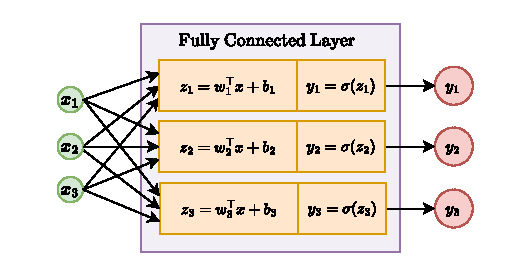
\includegraphics[width=0.7\linewidth]{Abschlussarbeit/Pictures/Layer_outp.pdf}
    \caption{Illustration of a neural networks layer}
    \label{fig:layer}
\end{figure}



A neural network consists of a set of artificial neurons, connected by directed and weighted connections, this is illustrated in Figure \ref{fig:IlNN}.
There are different layers shown, where each kind of layer has a different task: 
\begin{itemize}
   \item \textbf{Input layer} encodes the input values \( x_1, x_2, \dots, x_n \) and serves as the entry point of the network; it does not perform any computation itself.
    \item \textbf{Output layer} consists of a set of all output neurons, which represent the result with their output value
    \item \textbf{Hidden layer} consist of a set of all hidden neurons which belong neither to the input nor to the output layer
\end{itemize}


\begin{figure}[h]
    \centering
    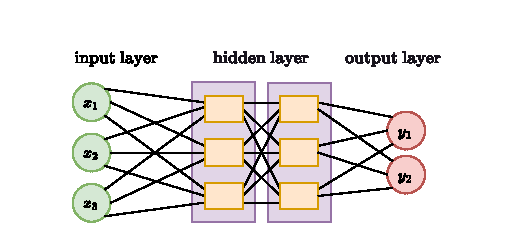
\includegraphics[width=0.7\linewidth]{Abschlussarbeit/Pictures/NN_mathematischausgerichtet.pdf}
    \caption{Illustration of a neural network. Adapted from \cite{zhou_machine_2021}.}
    \label{fig:IlNN}
\end{figure}


Further, we consider multilayer neural networks as in Cotterell et al.~\cite{cotterell_formal_2024}, where functions like those discussed above are composed.\\


Each function \( f^{(\ell)} : \mathbb{R}^{D^{(\ell-1)}} \rightarrow \mathbb{R}^{D^{(\ell)}} \), for \( \ell = 1, \dots, L \), represents a single layer of the network with \( D^{(\ell)} \) neurons.
The final layer \( f^{(L)} \) produces the networks output, so that the full network is defined as the composition:
\[
f = f^{(L)} \circ f^{(L-1)} \circ \dots \circ f^{(1)}.
\]

This composition defines a mapping \( f: \mathbb{R}^{D^{(0)}} \rightarrow \mathbb{R}^{D^{(L)}} \), where \(D^{(0)} \) is the number of input features, and \( D^{(L)} \) is the number of output neurons.

Each input \( x_n \in \mathbb{R}^{D^{(0)}} \), for \( n = 1, \dots, N \), is passed through the network to produce an output:
\[
y_n = f(x_n).
\]

The set \( \{ x_n \}_{n=1}^N \) is referred to as the feature space, and the corresponding outputs \( \{y_n \}_{n=1}^N \subset \mathbb{R}^{D^{(L)}} \) form the prediction space of the network. The total number of layers \( L \) is called the depth of the network.
